\begin{frame}{Training an MLLM in Stages}

  {\centering
  \resizebox{\textwidth}{!}{%
  \begin{tikzpicture}[font=\sffamily\scriptsize, >=latex,
      stagebox/.style={draw, rounded corners=0.1cm, align=left, text width=3.3cm, minimum height=2.0cm, inner sep=3pt},
      exnote/.style={align=left, text width=3.3cm, inner sep=3pt}]
    \node[stagebox, fill=blue!12] (s1) at (0,0) {\textbf{1. Alignment}\\[0.2em] trains: connector\\ frozen: encoder, LLM\\ data: image-caption pairs};
    \node[stagebox, fill=orange!16] (s2) at (4.0,0) {\textbf{2. Multimodal pretraining}\\[0.2em] trains: often all weights\\ data: captions, interleaved pages, OCR, VQA, text};
    \node[stagebox, fill=green!14] (s3) at (8.0,0) {\textbf{3. Instruction tuning}\\ (supervised fine-tuning, SFT)\\[0.2em] trains: LLM, connector\\ data: conversations, VQA, text-only chats};
    \node[stagebox, fill=red!10] (s4) at (12.0,0) {\textbf{4. Preference tuning}\\[0.2em] trains: LLM, connector\\ data: two answers per prompt, one marked preferred};
    \draw[->, thick] (s1) -- (s2);
    \draw[->, thick] (s2) -- (s3);
    \draw[->, thick] (s3) -- (s4);
    \node[exnote, anchor=north] (e1) at (0,-1.7) {trains its new (from-scratch) ViT, LLM frozen; captions, visual knowledge, OCR; 1.5T tokens};
    \node[exnote, anchor=north] (e2) at (4.0,-1.7) {all weights; adds interleaved, VQA, video, grounding, agent data; 2T tokens, then 0.6T at length 32{,}768};
    \node[exnote, anchor=north] (e3) at (8.0,-1.7) {about 2M samples, half of them text-only; ViT frozen};
    \node[exnote, anchor=north] (e4) at (12.0,-1.7) {image-text and text-only preference pairs, each used once; ViT frozen};
    \node[draw=black!50, dashed, rounded corners=0.1cm, inner sep=2pt, fit=(e1) (e2) (e3) (e4)] (ex) {};
    \node[anchor=south west, inner sep=1pt, font=\sffamily\scriptsize\bfseries] at (ex.north west) {Qwen2.5-VL};
  \end{tikzpicture}}\par}
  \vspace{0.3em}
  \begin{itemize}\footnotesize\itemsep0.3em
    \item \textbf{Curriculum:} an MLLM (multimodal LLM) meets harder data and longer inputs in later phases. Qwen2.5-VL packs 8{,}192-token sequences in its first two pretraining phases and 32{,}768-token sequences in the third.
    \item \textbf{Stages can merge:} InternVL3 starts from a pretrained base LLM but replaces stages 1 and 2 with one ``native multimodal pre-training'' stage that updates all weights on text-only and multimodal data together.
  \end{itemize}
  \vspace{0.1em}
  {\scriptsize Bai et al., ``Qwen2.5-VL Technical Report,'' 2025, \href{https://arxiv.org/abs/2502.13923v1}{arXiv:2502.13923v1}, Table~2 and Sections~2.2.2, 2.3.1, 2.3.4; Zhu et al., ``InternVL3: Exploring Advanced Training and Test-Time Recipes for Open-Source Multimodal Models,'' 2025, \href{https://arxiv.org/abs/2504.10479v3}{arXiv:2504.10479v3}, Sections~2.1 and~2.2.\par}
\end{frame}

\begin{frame}{Preference Tuning Against Hallucination}
  \begin{itemize}\footnotesize\itemsep0.3em
    \item \textbf{Preference tuning:} each sample is a prompt $x$ (image and question) with a preferred answer $y_w$ and a rejected one $y_l$, and the model learns to prefer $y_w$. \textbf{DPO} (Direct Preference Optimization) learns from the pairs directly. RLHF (reinforcement learning from human feedback) instead fits a reward model (a network that scores answers) to the pairs and then raises that score with reinforcement learning. The DPO loss:
    \[ \mathcal{L}_{\text{DPO}} = -\log \sigma\!\left(\beta \log \frac{\pi_\theta(y_w \mid x)}{\pi_{\text{ref}}(y_w \mid x)} - \beta \log \frac{\pi_\theta(y_l \mid x)}{\pi_{\text{ref}}(y_l \mid x)}\right) \]
    $\pi_\theta$: the model being tuned; $\pi_{\text{ref}}$: a frozen copy of the SFT model; $\sigma$: the logistic sigmoid; $\beta$: how strongly $\pi_\theta$ is held near $\pi_{\text{ref}}$ (larger $\beta$, closer). The loss is averaged over all pairs.
    \item \textbf{RLHF-V} builds pairs aimed at hallucination (text not grounded in the image): annotators rewrite only the wrong segments of a model's answer (1.4K answers), and a DPO variant gives the rewritten segments more weight.
  \end{itemize}
  \vspace{0.2em}
  {\centering\scriptsize
  \begin{tabular}{p{1.9cm} p{10.4cm}}
    \toprule
    $y_l$ (model) & The clock reads approximately \textcolor{red!75!black}{11:20} \ldots{} flags flying in the top \textcolor{red!75!black}{left} corner \ldots \\
    \addlinespace[0.2em]
    $y_w$ (annotator) & The clock reads approximately \textcolor{green!45!black}{15:26} \ldots{} flags flying in the top \textcolor{green!45!black}{right} corner \ldots \\
    \bottomrule
  \end{tabular}\par}
  \vspace{0.3em}
  {\scriptsize Rafailov et al., ``Direct Preference Optimization: Your Language Model is Secretly a Reward Model,'' NeurIPS 2023, \href{https://arxiv.org/abs/2305.18290v3}{arXiv:2305.18290v3}, Eq.~7; Yu et al., ``RLHF-V: Towards Trustworthy MLLMs via Behavior Alignment from Fine-grained Correctional Human Feedback,'' CVPR 2024, \href{https://arxiv.org/abs/2312.00849v2}{arXiv:2312.00849v2}, Sections~2 and~3.1 (Eq.~5); answer excerpts from its Figure~1.\par}
\end{frame}

\begin{frame}{Native Resolution and M-RoPE: Qwen2-VL}
  \begin{columns}[T,onlytextwidth]
    \column{0.52\textwidth}
      \begin{itemize}\footnotesize\itemsep0.3em
        \item \textbf{Native resolution:} no fixed square, no tiles. The 675M-parameter ViT reads each image at its own size and an MLP fuses each 2$\times$2 block of 14-pixel patch tokens, so the LLM gets one token per 28$\times$28 pixels: 64 for $224\times224$ (plus start and end markers), $25\times45 = 1{,}125$ for $700\times1260$. LLaVA-1.5 (without HD) always uses 576.
        \item \textbf{RoPE} (rotary position embedding) turns each pair of query and key features by an angle proportional to the token's position, so position enters attention scores only through the relative offset. Qwen2-VL's ViT uses a 2D version over patch rows and columns.
        \item \textbf{Video:} sampled at 2 frames per second; a 3D convolution of depth 2 merges each pair of frames, and an image enters as two identical frames. At most 16{,}384 tokens per training video.
      \end{itemize}
    \column{0.46\textwidth}
      \centering
      \vspace{0.2em}
      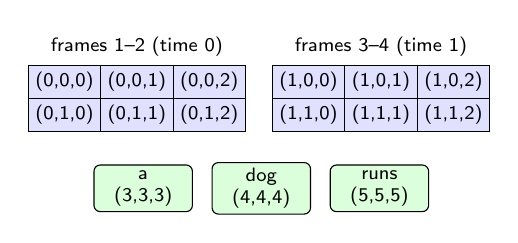
\begin{tikzpicture}[font=\sffamily\scriptsize,
          idcell/.style={draw, fill=blue!12, minimum width=0.92cm, minimum height=0.42cm, inner sep=1pt},
          wordbox/.style={draw, rounded corners=0.08cm, fill=green!14, minimum width=1.25cm, align=center, inner sep=2pt}]
        \foreach \rowi in {0,1} {
          \foreach \coli in {0,1,2} {
            \node[idcell] at ({0.92*\coli},{-0.42*\rowi}) {(0,\rowi,\coli)};
            \node[idcell] at ({3.1+0.92*\coli},{-0.42*\rowi}) {(1,\rowi,\coli)};
          }
        }
        \node at (0.92,0.45) {frames 1--2 (time 0)};
        \node at (4.02,0.45) {frames 3--4 (time 1)};
        \node[wordbox] at (1.0,-1.35) {a\\(3,3,3)};
        \node[wordbox] at (2.5,-1.35) {dog\\(4,4,4)};
        \node[wordbox] at (4.0,-1.35) {runs\\(5,5,5)};
      \end{tikzpicture}\\[0.4em]
      {\scriptsize\raggedright \textbf{M-RoPE} gives every LLM token three IDs (time, height, width), each driving its own share of the rotated feature pairs. Text gets three equal IDs, which is plain RoPE, and each new modality starts one above the largest ID so far: here a four-frame video (two merged frame pairs) of 2$\times$3 tokens, then text. A 25$\times$45-token image needs 45 position values where 1D RoPE would use 1{,}125.\par}
  \end{columns}
  \vspace{0.3em}
  {\scriptsize Wang et al., ``Qwen2-VL: Enhancing Vision-Language Model's Perception of the World at Any Resolution,'' 2024, \href{https://arxiv.org/abs/2409.12191v2}{arXiv:2409.12191v2}, Section~2.1, Figure~2 (token counts); diagram adapted from Figure~3. Su et al., ``RoFormer: Enhanced Transformer with Rotary Position Embedding,'' 2021, \href{https://arxiv.org/abs/2104.09864v5}{arXiv:2104.09864v5}.\par}
\end{frame}

\begin{frame}{Early Fusion Without a Vision Encoder}
  \begin{columns}[T,onlytextwidth]
    \column{0.52\textwidth}
      \begin{itemize}\footnotesize\itemsep0.3em
        \item \textbf{Early fusion:} images enter the token sequence at the first layer, with no CLIP-style encoder or connector (some texts also call LLaVA-style designs early fusion, since their visual tokens join the same sequence).
        \item \textbf{Fuyu-8B} (Adept, Oct.\ 2023): each 30$\times$30-pixel patch is linearly projected straight into a decoder-only Transformer, row by row, with an image-newline token after each row; any resolution works.
        \item \textbf{Chameleon} (Meta, 2024): a tokenizer with an 8{,}192-entry codebook (as in VQ-VAE) turns a 512$\times$512 image into 1{,}024 codes in the text vocabulary, so one model reads and writes images.
        \item \textbf{Stability:} shared weights let norms grow until training diverged; without QK-Norm (layer norm on queries and keys), Chameleon-7B diverged after about 20\% of an epoch.
        \item \textbf{Cost:} the tokenizer reconstructs text-heavy images poorly, which caps OCR-type tasks.
      \end{itemize}
    \column{0.46\textwidth}
      \centering
      \vspace{0.3em}
      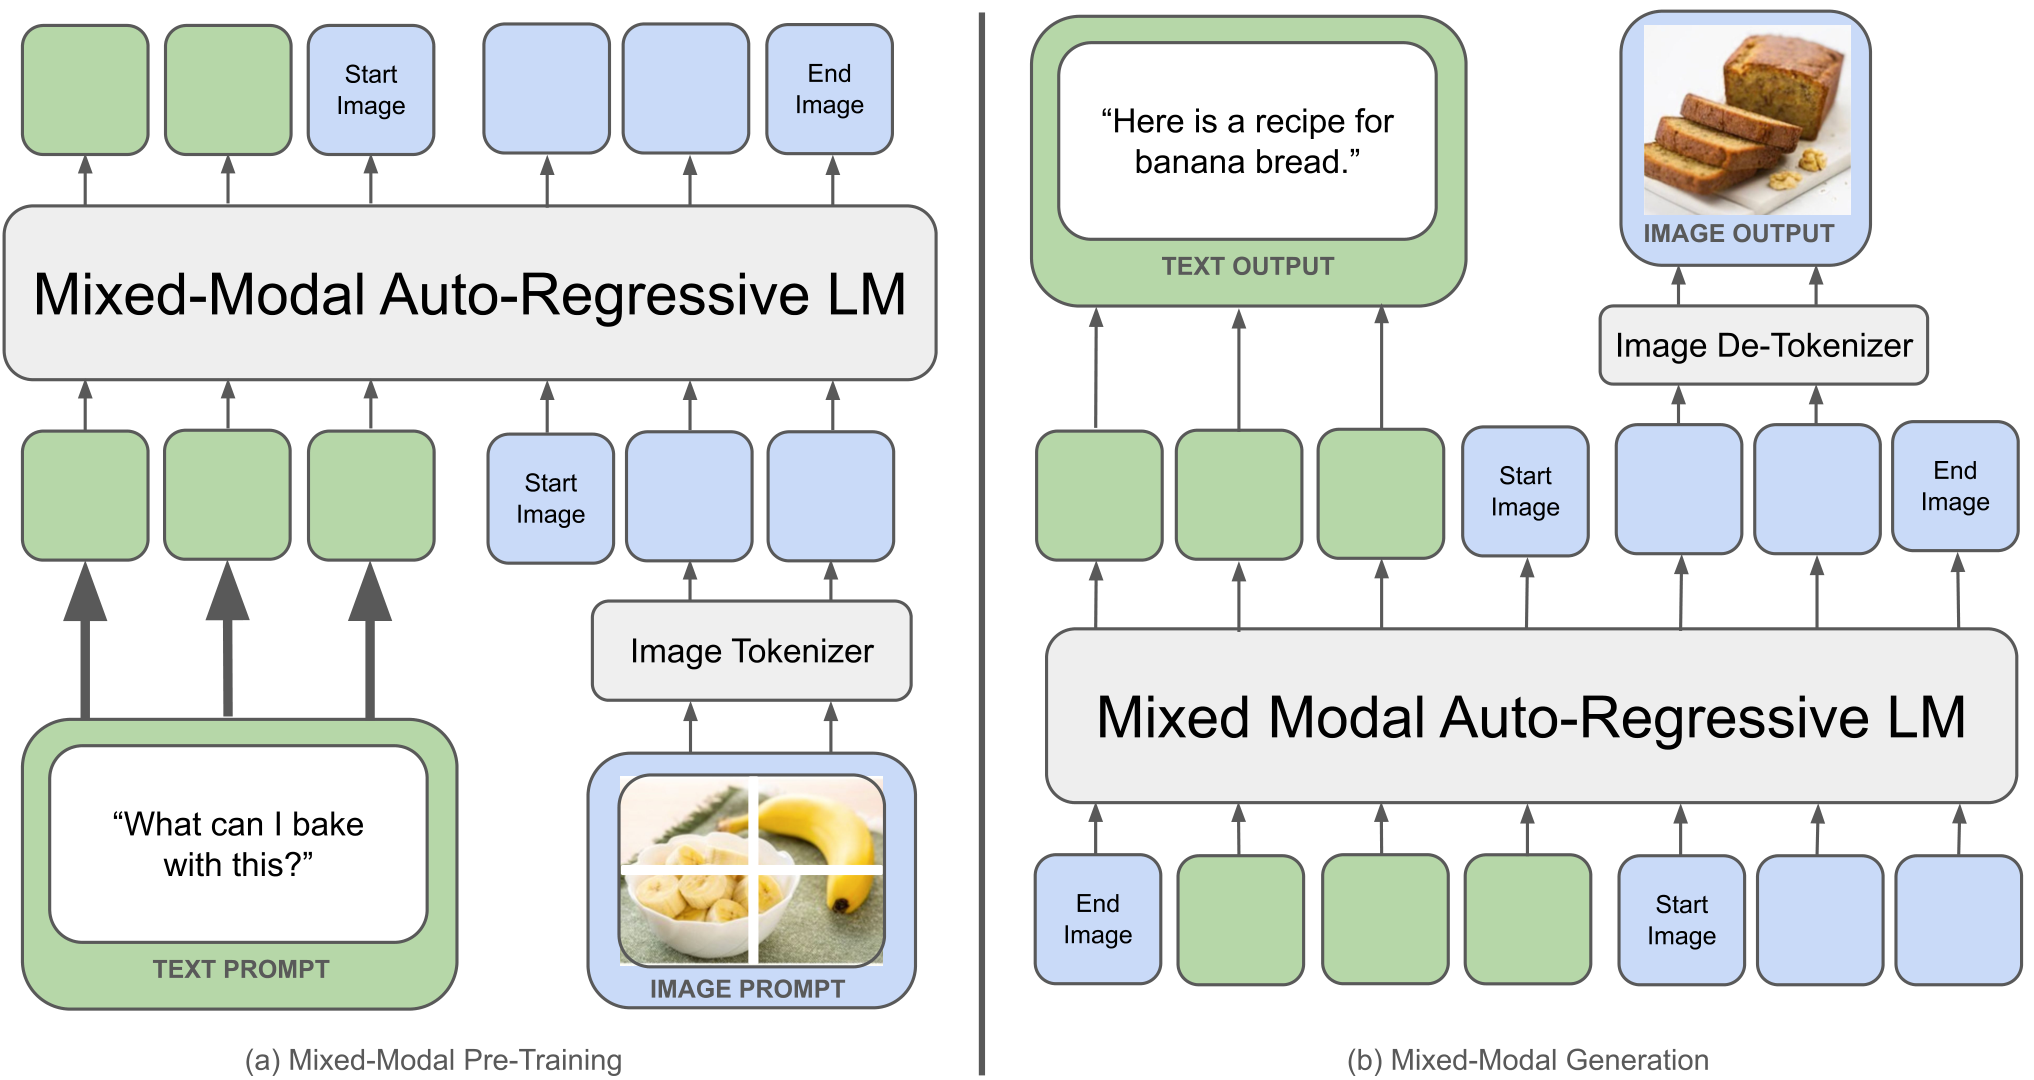
\includegraphics[width=\linewidth,height=0.46\textheight,keepaspectratio]{images/vision-language-models/chameleon_fig1_early_fusion.png}\\[0.2em]
      {\scriptsize Green: text tokens; blue: image tokens. (a) Mixed-modal pretraining on a text and an image prompt; (b) mixed-modal generation of text and an image. Chameleon Team, ``Chameleon: Mixed-Modal Early-Fusion Foundation Models,'' 2024, \href{https://arxiv.org/abs/2405.09818v2}{arXiv:2405.09818v2}, Figure~1; Sections~2.1 and~2.3.\par}
      \vspace{0.3em}
      {\scriptsize Fuyu-8B: Adept AI, model card and \texttt{config.json}, \href{https://huggingface.co/adept/fuyu-8b}{huggingface.co/adept/fuyu-8b}.\par}
  \end{columns}
\end{frame}

\begin{frame}{Grounding: Boxes and Points as Text Tokens}
  \begin{columns}[T,onlytextwidth]
    \column{0.52\textwidth}
      \begin{itemize}\footnotesize\itemsep0.3em
        \item \textbf{Kosmos-2} (Peng et al., 2023) links phrases to boxes (grounding) with one new token per cell of a $32\times32$ grid, 1{,}024 in all. A box is its top-left and bottom-right cells, placed after its phrase like a Markdown link. Cell $= 32\cdot\text{row} + \text{column}$, counting from 0, so \texttt{<loc44>} is row 1, column 12.
        \item \textbf{Qwen-VL} adds no location tokens: coordinates are scaled to $[0,1000)$ and written as plain text, as in \texttt{<ref>the ear on a giraffe</ref>} \texttt{<box>(176,106),(232,160)</box>}.
        \item \textbf{Qwen2.5-VL} uses the image's actual pixel coordinates for boxes and points, so the numbers also carry object size.
        \item \textbf{Scoring} referring expressions (RefCOCO and its variants): a box counts as correct if its IoU with the ground-truth box exceeds 0.5.
      \end{itemize}
    \column{0.46\textwidth}
      \centering
      \vspace{0.2em}
      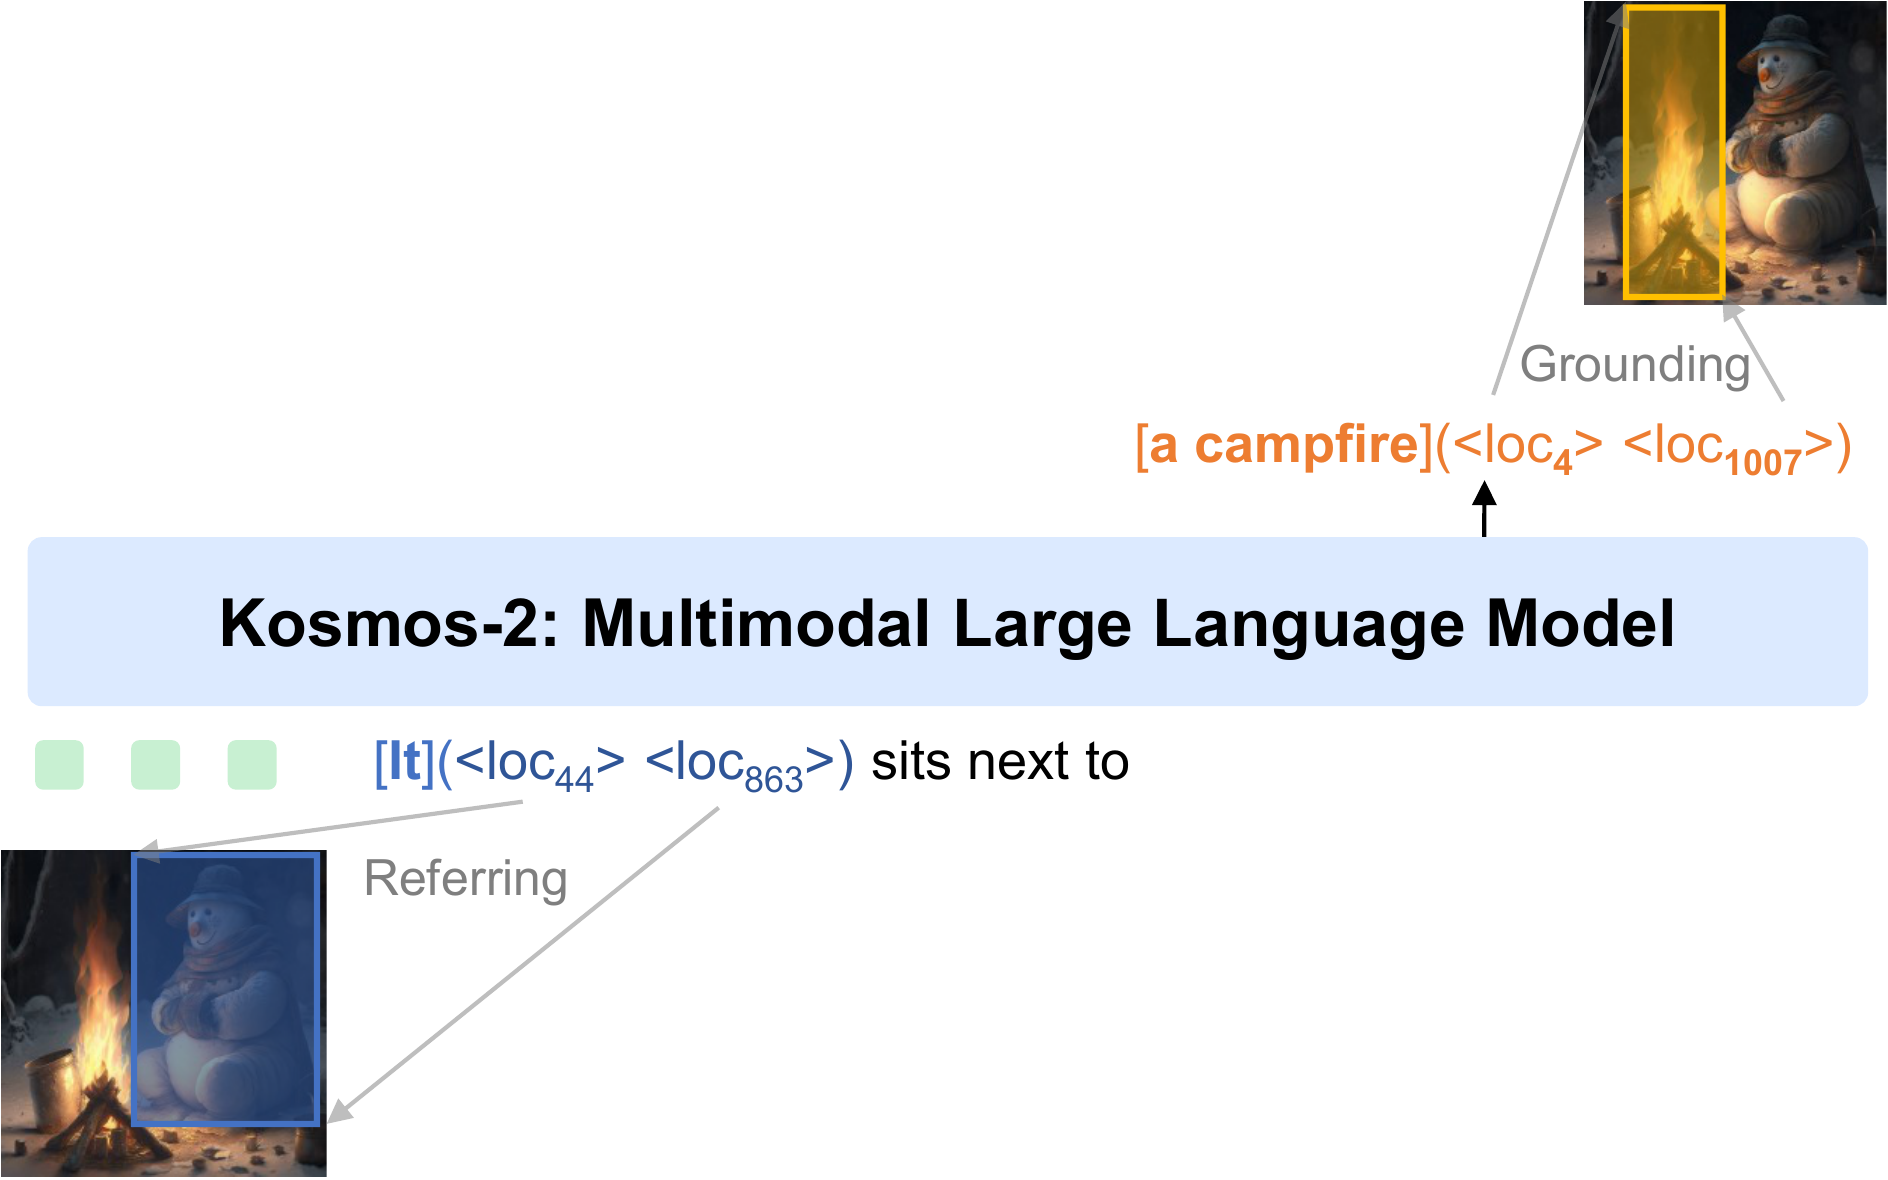
\includegraphics[width=\linewidth,height=0.46\textheight,keepaspectratio]{images/vision-language-models/kosmos2_fig1_location_tokens.png}\\[0.2em]
      {\scriptsize Peng et al., ``Kosmos-2: Grounding Multimodal Large Language Models to the World,'' 2023, \href{https://arxiv.org/abs/2306.14824v3}{arXiv:2306.14824v3}, Figure~1; Sections~3.1, 3.3 and~4.1.2.\par}
  \end{columns}
  \vspace{0.3em}
  {\scriptsize Cell order: Kosmos-2 decoding script, \href{https://github.com/microsoft/unilm/blob/97e4923e97d3ee10b57e97013556e3fd0d207a9b/kosmos-2/demo/decode_string.py}{github.com/microsoft/unilm}. Bai et al., ``Qwen-VL: A Versatile Vision-Language Model for Understanding, Localization, Text Reading, and Beyond,'' 2023, \href{https://arxiv.org/abs/2308.12966v3}{arXiv:2308.12966v3}, Section~2.2, Appendix~B.1; Qwen2.5-VL: \href{https://arxiv.org/abs/2502.13923v1}{arXiv:2502.13923v1}, Sections~2.1.2, 2.2.1.\par}
\end{frame}

\begin{frame}{Open-Weight MLLMs, 2024--2025: One Blueprint}

  {\centering\scriptsize\setlength{\tabcolsep}{3pt}
  \begin{tabular}{>{\raggedright\arraybackslash}p{1.9cm} >{\raggedright\arraybackslash}p{2.6cm} >{\raggedright\arraybackslash}p{2.3cm} >{\raggedright\arraybackslash}p{2.0cm} >{\raggedright\arraybackslash}p{4.0cm}}
    \toprule
    \textbf{Model} & \textbf{Vision encoder} & \textbf{Connector} & \textbf{LLM} & \textbf{Visual tokens per image} \\
    \midrule
    LLaVA-OneVision & SigLIP SO400M (384~px) & 2-layer MLP & Qwen2 0.5B, 7B, 72B & AnyRes: 384-px crops (grids up to 6$\times$6) plus the full view, 729 tokens each, interpolated down to $\leq 7{,}290$ in all \\
    \addlinespace[0.2em]
    Qwen2.5-VL & own ViT: window attention in most layers, 2D-RoPE & 2$\times$2 merge, 2-layer MLP & Qwen2.5 3B, 7B, 72B & native size: one per 28$\times$28 pixels \\
    \addlinespace[0.2em]
    InternVL3 & InternViT-300M or -6B (448 px) & pixel unshuffle (2$\times$2 into 1; InternVL 1.5 calls it pixel shuffle), 2-layer MLP & Qwen2.5 (0.5B--72B) or InternLM3-8B & 256 per 448-px tile; tile grid fitted to the aspect ratio (by default up to 12) plus a thumbnail \\
    \addlinespace[0.2em]
    Gemma 3 & SigLIP 400M (896 px), frozen & 4$\times$4 average pooling, linear map & Gemma 3 4B, 12B, 27B & 256 per 896-px view; at inference, Pan \& Scan splits large or non-square images into crops \\
    \bottomrule
  \end{tabular}\par}
  \vspace{0.3em}
  {\footnotesize Every row keeps LLaVA's layout. Beyond the choice of parts, the rows differ most in the visual-token budget and the last training step: instruction tuning for LLaVA-OneVision, DPO for Qwen2.5-VL, mixed preference optimization (DPO plus two more losses) for InternVL3, and distillation plus reinforcement learning for Gemma 3.\par}
  \vspace{0.3em}
  {\scriptsize Li et al., \href{https://arxiv.org/abs/2408.03326v3}{arXiv:2408.03326v3}; Bai et al., \href{https://arxiv.org/abs/2502.13923v1}{arXiv:2502.13923v1}; Zhu et al., \href{https://arxiv.org/abs/2504.10479v3}{arXiv:2504.10479v3} and the \href{https://huggingface.co/OpenGVLab/InternVL3-8B}{InternVL3-8B model card}; Gemma Team, \href{https://arxiv.org/abs/2503.19786v1}{arXiv:2503.19786v1}, and \href{https://github.com/huggingface/transformers/blob/v4.50.0/src/transformers/models/gemma3/modeling_gemma3.py}{Transformers v4.50.0} (linear map).\par}
\end{frame}
